\documentclass[../talk.tex]{subfiles}
\begin{document}

\begin{frame}{Certificates}
    \begin{overlayarea}{\slidewidth}{\slideheight}
        \begin{center}
            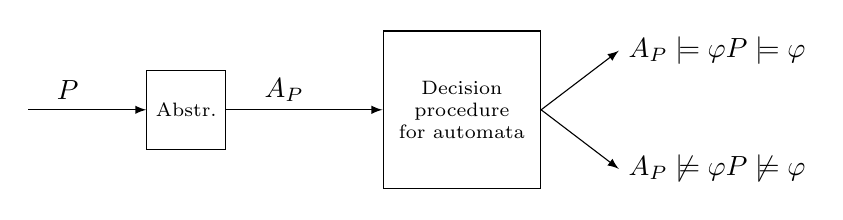
\begin{tikzpicture}
                \node (origin) [coordinate] at (0.5,0) {};

                \node (abstr) at (2,0) [minimum width=1cm, minimum height=1cm, anchor=west,draw] {};

                \node (rect) at (5,0) [minimum width=2cm,minimum height=2cm, anchor=west,draw] {};

                \node (yes) [coordinate] at (8,0.75) {};
                \node (no) [coordinate] at (8,-0.75) {};
                \path [->,>=latex]
                    (origin) edge (abstr.west)
                    (abstr.east) edge (rect.west)
                    (rect.east) edge (yes)
                    (rect.east) edge (no)
                ;

                \node at (1,0.25) {$P$};

                \node at (3.75,0.25) {$A_P$};

                \node [right of=yes, node distance=0cm, anchor=west] {$A_P \models \varphi \implies P \models \varphi$};
                \node [right of=no, node distance=0cm, anchor=west] {$A_P \not\models \varphi \implies P \not\models \varphi$};

                \node [align=center, text width=1cm, font=\scriptsize] at (abstr) {Abstr.};
                \node [align=center, text width=2cm, font=\scriptsize] at (rect) {Decision procedure for automata};
            \end{tikzpicture}
        \end{center}

        \vspace*{-1em}
        This is too optimistic!

        \vspace*{1em}

        \sonslide<2->%
        {%
            Problem: We assume that a \alert{boolean (yes/no)} answer to the decision problem is sufficient

            \vspace*{1em}
        }

        \sonslide<3->%
        {%
            Need more detailed output!

            \begin{itemize}
                \sitem<4->[$-$] \alert{Accountability}: We don't want to trust the algorithm blindly
                \sitem<5->[$-$] We often need \alert{more than one call} of a decision procedure
                \sitem<6->[$-$] Later calls need information computed by earlier ones
                    \newline
                    e.g.~compositional verification, refinement loops (CEGAR)
            \end{itemize}
        }
    \end{overlayarea}
\end{frame}

\end{document}
